% Chapter Template

\chapter{Estructura del mutualismo} % Main chapter title
\label{ESTATICA} % Change X to a consecutive number; for referencing this chapter elsewhere, use \ref{ChapterX}

%----------------------------------------------------------------------------------------
%	SECTION 1
%----------------------------------------------------------------------------------------

\section{Propiedades estructurales del mutualismo}

Lorem ipsum dolor sit amet, consectetur adipiscing elit. Aliquam ultricies lacinia euismod. Nam tempus risus in dolor rhoncus in interdum enim tincidunt. Donec vel nunc neque. In condimentum ullamcorper quam non consequat. Fusce sagittis tempor feugiat. Fusce magna erat, molestie eu convallis ut, tempus sed arcu. Quisque molestie, ante a tincidunt ullamcorper, sapien enim dignissim lacus, in semper nibh erat lobortis purus. Integer dapibus ligula ac risus convallis pellentesque 

%-----------------------------------
%	SUBSECTION 1
%-----------------------------------
\subsection{Magnitudes clásicas}

Nunc posuere quam at lectus tristique eu ultrices augue venenatis. Vestibulum ante ipsum primis in faucibus orci luctus et ultrices posuere cubilia Curae; Aliquam erat volutpat. Vivamus sodales tortor eget quam adipiscing in vulputate ante ullamcorper. Sed eros ante, lacinia et sollicitudin et, aliquam sit amet augue. In hac habitasse platea dictumst.

\section{Descripción basada en la descompisión \textit{k-core}}

La \textit{descomposición k-core}\footnote{Utilizamos la expresión original en inglés por ser prevalente en la bibliografía, a pesar de que algunos autores han propuesto traducciones como textit{núcleos de grado k} \cite{herrero2000terminologia} o \textit{k-núcleos} \cite{cardona2006taxonomia, martinez2011aplicacion}} fue utilizada por primera vez por Stefen Seidman para medir la densidad local y la cohesión en redes sociales \cite{seidman1983network}. Dado un grafo no dirigido, un \textit{k-core} es el subgrafo máximo el el que todos sus nodos están conectados con al menos otros $k$ puntos \cite{dorogovtsev2006k}.

\begin{theo} 
Sea un grafo no dirigido $G = \{V, E\}$, donde $V$ y $E$ son los conjuntos de nodos y enlaces respectivamente. Llamamos $deg_G(v)$ al grado del nodo $v$ en el grafo $G$. El subgrafo $M = \{C, E|C\}$ inducido por el subconjunto de nodos $C \subseteq V$ es
un $k$-$core$ si $\forall v \in C: \big( deg_G(v) \geq k \big)$ y $M$ es el subgrafo máximo que cumple la condición. Se denomina $k$-$shell$ al conjunto de nodos del $k$-$core$ que no pertenecen al $k+1$-$core$.
\label{ESTATICA_def_kcore}
\end{theo}

La \textit{descomposición k-core} se ha utilizado de forma habitual como mecanismo de reducción de información para estudiar redes de distinta naturaleza \cite{kitsak2010identification, zhang2010using, barbera2014critical}. El resultado ofrece una visión organizada en capas, con los nodos más centrales en la \textit{shell} de mayor $k$. Esta cifra puede llegar al orden de las centenas en redes grandes. Hasta donde nosotros sabemos, no hay literatura sobre su aplicación al estudio del mutualismo, ya que son redes bipartitas de un tamaño mínimo comparado con los sistemas sociales o tecnológicos a los que se ha aplicado.

Existen diversos algoritmos para llevar a cabo la descomposición en función de las dimensiones de la red\cite{montresor2013distributed}. El más sencillo y válido para el caso de las redes mutualistas, es el algoritmo de podado (\textit{pruning}), que se describe con la ayuda de la figura \ref{fig:ESTATICA_kcore_decomposition_example}, una red bipartita ficticia, con ocho nodos de una clase y siete de la opuesta. A la hora de aplicar el algoritmo resulta irrelevante que la red sea bipartita, pues solo se basa en el número de enlaces y no en la naturaleza de los nodos que conectan.

Se empieza eliminando enlaces de aquellos nodos que solo tienen un enlace, por ejemplo el que une el nodo de color verde número 8 con el de color chocolate número 4. Se sigue realizando la operación mientras queden nodos con un único enlace, hasta que llegue el momento en que todos los nodos restantes tengan dos o más. Los nodos que han quedado desconectados forman la \textit{1-shell}. Repetimos el procedimiento para dos enlaces y así sucesivamente, clasificando todos los nodos en su \textit{shell} correspondiente. En este ejemplo sencillo el $k$ máximo es 3. Nótese que cada nodo pertenece a una $shell$.

\begin{figure}[h!]
\centering
\includegraphics[scale=0.5]{Figures/ESTATICA_kcore_decomposition_example.png}
\caption[PolarExample]{Descomposición \textit{k-core} de una red bipartita ficticia.}
\label{fig:ESTATICA_kcore_decomposition_example}
\end{figure}

Según la definición \ref{ESTATICA_def_kcore}, el  \textit{1-core} es la unión de las tres \textit{shell}, mientras que el \textit{2-core} es la unión de la \textit{2-shell} y la \textit{1-shell}. El \textit{k-core} máximo coincide con la  \textit{k-shell} máxima. 

Como estamos tratando de redes bipartitas, distinguimos dos subconjuntos en cada \textit{k-shell}, el de los nodos de la clase $A$ y el de los de la clase $B$. Los llamaremos $K^{A}_{j}, K^{B}_{j}$, donde  $j$ es el índice de la \textit{k-shell}.
Es posible que uno de ellos sea vacío, es decir, no todas las \textit{k-shell} tienen nodos de ambas clases necesariamente.
Al valor máximo de \textit{k}, lo llamamos $ks_{max}$, que corresponde a \textit{shell} más interna de la red $ks_{max}\equiv C^{A,B}$. Esta nomenclatura simplifica la definición de las \textit{k-magnitudes} que surgen de la red descompuesta siguiendo el procedimiento descrito.


\section{K magnitudes}

Las especies más conectadas de una red mutualista son resistentes a las perturbaciones externas porque el beneficio que reciben depende de múltiples fuentes. Esta parece ser la razón por la que las redes mutualistas tienden al anidamiento, una conexión directa con el centro de la red aumenta las probabilidades de supervivencia. Para medir la 'distancia' desde un nodo cualquiera a la \textit{k-shell} más interna de la clase opuesta, hemos definido el \textit{$k_{radius}$}.

\begin{theo} 
El \textit{$k_{radius}$} del nodo $m$ de la clase $A$ es el valor medio de la distancia a las especies de $C^B$.
\begin{align*}
\displaystyle
k^A_{radius}m = \frac{1}{\mid C^{B} \mid}\sum\limits_{j \in C^{B}} dist_{mj}  \qquad   m \in A
\stepcounter{equation}\tag{\theequation}\label{kradius}
\end{align*}
\label{ESTATICA_kradius}
\end{theo}

En la fórmula \ref{ESTATICA_kradius} $dist_{mj}$ es el camino más corto de la especie $m$ a cada una de las $j$ especies que forman el conjuto $C^B$. La misma definción es válida para especies de la clase $B$, calculando la distancia media a las especies de $C^A$. El valor mínimo posible de $k_{radius}$ es $1$ para un nodo perteciente a $C^B$ conectado con todas las especies de $C^A$ (y viceversa).

\begin{figure}[h!]
\centering
\includegraphics[scale=0.5]{ESTATICA_red_example.eps}
\caption {Cálculo de \textit{$k_{radius}$} y  \textit{$k_{degree}$} en una red ficticia.}
\label{fig:ESTATICA_red_example}
\end{figure}

La parte superior izquierda de la figura \ref{fig:ESTATICA_red_example} es el esquema de otra red ficticia muy sencilla, con solo siete nodos, tres de la clase $A$ y cuatro de la $B$. La descomposición $k$-$core$ indica que la especie $B4$ es la única de la $1$-$shell$. El resto pertenecen a la $2$-$shell$, que por ser la más interna sirve de base para medir el $k_{radius}$. 

En la parte superior derecha de la imagen, se reproduce el detalle de las conexiones de la especie $A1$, perteneciente a $C^{A}$.  Como está directamente conectada con los tres nodos de $C^{B}$ la el camino más corto a cada uno de ellos es $1$, y en consecuencia $k^A_{radius}1$ es $1$. En la parte inferior derecha, la especie $A2$ que también pertenece a $C^{A}$ no tiene enlace directo con $B2$, aunque sí con $B1$ y $B3$. El camino más corto, marcado en color violeta, pasa por $B1$ y $A1$, y mide $3$. El $k^A_{radius}2$ vale $\frac{5}{3}$. En la parte inferior izquierda, vemos el esquema de conexiones de la especie $B4$, que no forma parte de $C^{B}$. Como cabía esperar, su$k_{radius}$ es mayor, $\frac{7}{3}$. 

Podemos definir una magnitud global, teniendo en cuenta los $k_{radius}$ de todas las especies.

\begin{theo} 
El \textit{$\overline k_{radius}$} de una red se obtiene promediando los ${k}_{radius}$ de todos los nodos, sin importar la clase a la que pertenezcan.

\begin{align*}
\displaystyle
\overline {k}_{radius} = \frac{1}{\mid A \cup B \mid}\sum\limits_{l \in A \cup B} k_{radius}l
\stepcounter{equation}\tag{\theequation}\label{avgkradius}
\end{align*}
\label{ESTATICA_avgkradius}
\end{theo}

Una red con todos sus nodos conectados (matriz de adyacencia cuadrada) tendría $\overline {k}_{radius}=1$, el menor posible. En una con matriz de adyacencia triangular el $\overline {k}_{radius}$ vale $1.5$. En la red que hemos usado como ejemplo, su valor es $\frac{11}{7}$. Intuitivamente, el $\overline {k}_{radius}$ será pequeño para redes muy anidadas, porque la probabilidad de conexión con la \textit{shell} más interna es elevada. Las especies generalistas están muy interconectadas y las especialistas tienen enlaces directos con las \textit{k-shells} de mayor índice. por el contrario, una distribución de enlaces puramente aleatoria conduciría a una red con mayor $\overline {k}_{radius}=1$.

El ${k}_{radius}$ es una buena medida de conexión al núcleo central pero no de centralidad. Por ejemplo, su valor es bajo para un especialista con un enlace a la \textit{shell} más interna, aunque sabemos que no resulta determinante para la estabilidad global de la red. Para atender esta necesidad, definimos una segunda \textit{k-magnitud}.

\begin{theo} 
\begin{align*}
\displaystyle
k^A_{degree}m = \sum\limits_{j} \frac{a_{mj} }{k_{radius}j}  \quad   m \in A, \forall j \in B
\stepcounter{equation}\tag{\theequation}
\end{align*}
\label{kdegree}
\end{theo}

Donde $a_{mj}$ es el elemento de la mtriz de interacción que representa el enlace, cuyo valor es $1$ si existe o $0$ si no está presente. El $k_{degree}$ es la suma de los inversos de los $k_{radius}$ de los nodos conectados con$m$. Una especie de la \textit{shell} más interna tiene un $k_{degree}m$ elevado,  mientras que los especialistas con solo uno o dos enlaces tiene un $k_{degree}$ reducido. Volviendo al ejemplo de la figura \ref{fig:ESTATICA_red_example}, el $k_{degree}$ del nodo $B3$ es is $1+3/5+3/5 = 11/5$, mientras que solo vale $3/7$ para el especialista $B4$. Esta magnitud recuerda la definición del \textit{índice de Harary} \cite{plavvsic1993harary} pero teniendo solo en cuenta los enlaces con la \textit{shell} más interna.


\subsection{Algoritmo de destrucción basado en \textit{k-shell}}

Para poder establecer políticas de conservación es necesario disponer de un respaldo cuantitativo. La biodiversidad y resistencia de una comunidad mutualista depende de la estructura de la red de interconexiones. La extinción de algunas especies provoca que partes de la red queden desconectadas de la componente gigante y posiblemente expuestas a la desaparición. Por este motivo, la evolución del tamaño de la componente gigante cuando se eliminan especies es el criterio más utilizado para estudiar la resistencia estructural estática de las comunidades de población.

Esto es lo que hace el método de medida de Dunne \cite{dunne2002biodiversity}. Las especies se van retirando una por una de la red (extinciones primarias). Este hecho produce extinciones secundarias de aquellas especies que resultan desconectadas de la componente gigante. La gráfica de la fracción de la componente gigante inicial superviviente, frente a la fracción de extinciones primarias (en escala normalizada entre 0 y 1) define la \textit{curva de extinción}. Cuanto menor sea el área bajo esta curva, más rápida será la destrucción de la red.

\begin{figure}[h!]
\centering
\includegraphics[scale=0.55]{Figures/ESTATICA_destruction_example.png}
\caption[PolarExample]{Ejemplo de gráfica de destrucción siguiendo el método de Dunne. El área bajo la curva indica la velocidad a la que se desintegra la componente gigante.}
\label{fig:ESTATICA_destruction_example}
\end{figure}

La clave está en el orden de selección de las especies que se retiran en las extinciones primarias. Si disponemos de una cifra que defina su importancia para esa red concreta, se podrán concentrar los esfuerzos de conservación en las especies que más aportan a la supervivencia del sistema. El problema es que no existe un criterio único para establecer esa clasificación, por lo que es un campo de investigación activo \citep{dominguez2015ranking}.

En el mutualismo, parece lógico pensar que las especies de las \textit{shells} más internas son las más importantes para mantener la integridad de la red. El algoritmo de destrucción que proponemos se basa en la secuencia $k$-$shell$/$k_{degree}$/$k_{radius}$, esto es, se empiezan las extinciones primarias por las especies pertenecientes a la $k$-$shell$ de mayor índice, y dentro de esta, el de mayor $k_{degree}$, y en caso de coincidencia, el de menor $k_{radius}$. Como veremos en la sección de resultados esta selección es muy eficaz comparada con el algoritmo más eficaz de los publicados. 


\section{Resultados}

Nunc posuere quam at lectus tristique eu ultrices augue venenatis. Vestibulum ante ipsum primis in faucibus orci luctus et ultrices posuere cubilia Curae; Aliquam erat volutpat. Vivamus sodales tortor eget quam adipiscing in vulputate ante ullamcorper. Sed eros ante, lacinia et sollicitudin et, aliquam sit amet augue. In hac habitasse platea dictumst.

\begin{figure}[hbp!]
\centering
\includegraphics[scale=0.18]{Figures/ESTATICA_tamanyo_kdegree_kradius.png}
\caption[PolarExample]{Ejemplo de gráfica de destrucción siguiendo el método de Dunne. El área bajo la curva determina la velocidad a la que se desintegra la componente gigante.}
\label{fig:ESTATICA_tamanyo_kdegree_kradius}
\end{figure}

\subsection{Análisis exploratorio}

En una primera aproximación visual encontramos que existe una alta correlación entre el $\overline{k}_{radius}$ de la red y el número de especies (figura \ref{fig:ESTATICA_tamanyo_kdegree_kradius}). Como cabía esperar, cuanto mayor es la red, mayor es la distancia media a la \textit{shell} máxima. El crecimiento sigue una ley logarítmica, nótese la escala del eje $X$. Sucede algo parecido con el número de enlaces, pero en este caso se puede apreciar mayor dispersión. 

Por el contrario, el $\overline{k}_{degree}$ no parece guardar ninguna relación con el tamaño de la red, ya se mida en número total de especies o de enlaces. Vemos que para la mayoría de redes su valor está en torno a $2$. Este dato hace sospechar que la distribución del $\overline{k}_{degree}$ sigue una exponencial decreciente. La mayoría de los nodos tienen valores muy bajos, por lo que la media arroja ese valor tan pequeño.

Si observamos la relación entre las dos \textit{k-magnitudes} y el indíce $k$ máximo de la red, descubrimos que la relación es inversa, el $\overline{k}_{degree}$ crece con el índice y el $\overline{k}_{radius}$ disminuye. No obstante, se aprecia una importante dispersión para redes con un mismo $k$ máximo.

\subsection{Correlación entre \textit{k-magnitudes} y propiedades globales}

Uno de los objetivos principales de la investigación es hallar la posible relación entre las magnitudes que se derivan de la \textit{descomposición k-core} y las que se utilizan habitualmente en la caracterización del mutualismo \textit{anidamiento} y \textit{modularidad}. Hemos encontrado que las \textit{k-magnitudes} globales tienen una fuerte correlación con estas dos medidas, y esto es de gran interés puesto que surgen de la agregación de las propiedades locales de cada nodo.

Para realizar la comparación se calcula el anidamiento mediante \textit{NODF} \cite{almeida2008consistent} y la modularidad siguiendo la definición de \textit{Modularity} de Newman \cite{newman2004finding} \footnote{Para evitar confusiones entre el nombre la de la magnitud y la medida según un algoritmo concreto, en lo sucesivo se emplea \textit{Modularity}, en inglés y con mayúscula, para referirse al valor definido por Newman.}. Ambas medidas las proporciona el paquete \texttt{bipartite} en \texttt{R}. En la figura \ref{fig:ESTATICA_corrfigs} se han representado el $\overline {k}_{radius}$ en función de $NODF$ y el $\overline {k}_{degree}$ en función de la $modularidad$. Las figuras sugerían que existe un fuerte correlación negativa entre el $\overline {k}_{radius}$ y $NODF$ por una parte y, por otra, entre el $\overline {k}_{degree}$ y la $modularidad$. 

\begin{figure}[h!]
\centering
\includegraphics[scale=0.2]{ESTATICA_correlation_figs.png}
\caption {Diagrama de dispersión del $\overline {k}_{radius}$ respecto a $NODF$ (izquierda), y del $\overline {k}_{degree}$ respecto a la $Modularity$ (derecha). Cada punto es una red, su área es proporcional al logaritmo del número de especies y el color indica la clase de comunidad. Se han incluido las líneas de regresión con sus intervalos de confianza en sombreado.}
\label{fig:ESTATICA_corrfigs}
\end{figure}

Las nubes de puntos se represntan sobre eje lineal en las abscisas y logarítmico en las ordenadas. Parecen compatibles con un modelo exponencial, así que procedimos a calcular las regresiones lineales $log(Y) ~ X$. Los resultados numéricos se resumen en la tabla \ref{table:table_lmodel}. Como muestra el valor ajustado de $R^2$ $(0.84)$, el logaritmo de $\overline {k}_{radius}$ tiene una correlación muy elevada con $NODF$ por lo quenitid. Es sencillo de entender, porque si la red es muy anidada las especies se conectan directamente a las \textit{shells} más internas y su distancia a los nodos de la \textit{shell} máxima es pequeña. 

\begin{table}[ht]
\centering
\begin{tabular}{|l r | l r|}
\hline
$log(\overline {k}_{radius})$ vs $NODF$& & $log(\overline {k}_{degree})$ vs $Modularity$ & \\
\hline
$\beta_1$ & $-$0.0098 & $\beta'_1$ & -2.5031 \\
$\beta_0$ & 1.2269 & $\beta'_0$ & 1.5553 \\
Adjusted $R^2$ &  0.8427  & Adjusted $R'^2$& 0.8064\\
p-value & $<2.2 \times 10^{-16}$& p-value' & $<2.2 \times 10^{-16}$\\
\hline
\end{tabular}
\caption{\label{table:table_lmodel} Linear regression results}
\end{table}

La fuerte correlación entre $\overline {k}_{degree}$ y $Modularity$ es más complicado intuirla. La distribución de densidad del $k_{degree}$ está más concentrada y sesgada hacia la izquierda cuanto más modular es la red. En ese caso la mayoría de las especies tienen valores reducidos del ${k}_{degree}$ y en consecuencia el valor medio es reducido. La distribución se va aplanando a medida que la modularidad decrece y el valor medio se desplaza hacia la derecha. En la figura \ref{fig:ESTATICA_density_plots} se puede ver este efecto.

Si se examina de nuevo la figura \ref{fig:ESTATICA_corrfigs}, se verá que las redes de mayor tamaño son también las que tienen valores más altos de $Modularity$. La mayoría de ellas son de la clase \textit{plata-polinizador} mientras que las tipo \textit{dispersor de semillas} son más pequeñas. Este hecho ya fue puntado por Olesen que estudió 51 redes y encontró que las que tienen menos de 150 especies no son modulares \cite{olesen2007modularity}. Los valores elevados de $\overline {k}_{degree}$ en redes reducidas casan bien con la observación de que en ese caso las especies se encuentran más próximas a la \textit{shell} más interna y añaden valores altos al ${k}_{degree}$ de las especies a las que se conectan.

Las elevadas correlaciones de $\overline {k}_{radius}$ con $NODF$ y de $\overline {k}_{radius}$ con $Modularity$ son suficientes para esta investigación. Por ejemplo, no se propugna que $log(\overline {k}_{radius})$ sea un buen predicto de $NODF$, de hecho el test de \textit{Shapiro-Wilk} muestra Heterocedasticidad. La colección de la \textit{Web of Life} no es una muestra aleatoria, y la distribución de las magnitudes no son normales. Sin embargo, las correlaciones apoyan la idea de que el $\overline {k}_{radius}$ es un indicador global de anidamiento, y el $\overline {k}_{degree}$ de modularidad y que la \textit{descomposición k-core} es una alternativa válida para el estudio del mutualismo.

\begin{figure}[h!]
\centering
\includegraphics[scale=1]{ESTATICA_density_plots.png}
\caption {Distribución de densidad del $k_{degree}$ en tres redes diferente. Junato a las líneas verticales pueden verse los valores del $\overline {k}_{degree}$ y de la $Modularity$.}
\label{fig:ESTATICA_density_plots}
\end{figure}

\subsection{Recableado aleatorio}

\section{Conclusiones}

Nunc posuere quam at lectus tristique eu ultrices augue venenatis. Vestibulum ante ipsum primis in faucibus orci luctus et ultrices posuere cubilia Curae; Aliquam erat volutpat. Vivamus sodales tortor eget quam adipiscing in vulputate ante ullamcorper. Sed eros ante, lacinia et sollicitudin et, aliquam sit amet augue. In hac habitasse platea dictumst.
